\documentclass[11pt]{article}
\usepackage[T1]{fontenc}
\usepackage{lmodern,amsmath,amssymb,amsthm,mathtools,booktabs,longtable,tabularx,array}
\usepackage[margin=0.9in]{geometry}
\usepackage{microtype,xcolor,graphicx,enumitem,xurl,hyperref,fancyhdr}
\definecolor{ink}{HTML}{173A52}
\definecolor{accent}{HTML}{146C78}
\hypersetup{colorlinks=true,linkcolor=ink,citecolor=accent,urlcolor=accent,
pdftitle={Beyond Dirichlet GRH: exact torsion specialization and the limits of transfer},
pdfauthor={Research memorandum for Vladimir Reshetnikov}}
\setlength{\emergencystretch}{2em}
\setlength{\headheight}{14pt}
\pagestyle{fancy}\fancyhf{}
\fancyhead[L]{\small Beyond Dirichlet GRH}
\fancyhead[R]{\small 25 November 2026}
\fancyfoot[C]{\thepage}
\newtheorem{theorem}{Theorem}[section]
\newtheorem{lemma}[theorem]{Lemma}
\newtheorem{proposition}[theorem]{Proposition}
\newtheorem{corollary}[theorem]{Corollary}
\theoremstyle{definition}\newtheorem{definition}[theorem]{Definition}
\newcommand{\Q}{\mathbb Q}
\newcommand{\Z}{\mathbb Z}
\newcommand{\C}{\mathbb C}
\newcommand{\R}{\mathbb R}
\newcommand{\Rea}{\operatorname{Re}}
\newcommand{\ord}{\operatorname{ord}}
\newcommand{\length}{\operatorname{length}}
\newcommand{\G}{\mathsf G}
\newcommand{\Sha}{\mathrm{Sha}}
\newcommand{\src}[1]{\texttt{\small #1}}
\title{\color{ink}\bfseries Beyond Dirichlet GRH\\[5pt]
\Large Exact torsion specialization and the limits of transfer}
\author{Research memorandum for Vladimir Reshetnikov\\
\small Source analysis, complete mathematical proofs, and reproducible checks}
\date{25 November 2026}
\begin{document}
\maketitle
\begin{abstract}
The proof in \texttt{lsernau/grh-lean} contains reusable mathematics beyond its
RH and Dirichlet-GRH conclusions. Its central construction compares upper and
lower bounds for the same covolume of iterated theta lifts; its auxiliary
arguments select roots of unity with controlled valuations and bound
congruence denominators. After reviewing the 26 earlier incoming ProveIt
archives, we develop an exact specialization theorem: an integral polynomial
or bounded integral power series of fixed positive-radius Gauss valuation at
most \(B\) admits a \(p\)-power torsion specialization of no larger valuation,
with the explicit order-exponent bound
\(H=h_0+\lceil p^{h_0}B(h_0+B+2)\rceil\).
The same bound per coordinate works in any finite dimension and controls the
total valuation of a packet, independently of its cardinality. Two
counterexamples show why exact individual bounds and an exact moving-radius
comparison cannot be inferred. The proof is complete on paper; finite checks
use exact arithmetic, and no new Lean verification is claimed.
We also distinguish the shortened proof from the original Step-17 input used
in recent \(K\)-theory applications, and specify the missing arithmetic input
for a nonabelian RH benchmark. We do not claim a new solution of Vandiver,
BSD, Artin's primitive-root conjecture, or a nonabelian RH instance. The new
specialization bound is an extension relative to the inspected reports;
worldwide priority is not established.
\end{abstract}
\clearpage
\tableofcontents
\newpage
\section{Answer to the research question}
\label{sec:assessment}

Yes: the proof's methods have meaningful applications beyond familiar
consequences of the truth of RH and Dirichlet GRH. There are, however, three
different kinds of result to distinguish.

First, the original Alp\"oge--Claude proof contains a strict Selmer estimate
that recent authors have used to claim new finite-range algebraic
\(K\)-group vanishings. This is a genuine transfer of an internal arithmetic
argument, rather than an implication of the statement of RH. The relevant
term belongs to the original large archive; it is not the
\src{exists\_length\_shaOdd\_le} term in the shortened repository.
Mok--Zheng's 24 November preprint claims vanishing through degree \(120\),
and explicitly records an incomplete rebuild of its modified Lean entry
point \cite{mokzheng}. This report does not independently certify that result.

Second, the shortened proof's torsion-selection mechanism yields a concrete
result proved in this report. Let \(v(p)=1\), let \(\mathcal O\) be the
valuation ring of \(\C_p\), and write
\[
 \G_\rho(F)=\min_\nu\{v(a_\nu)+\rho|\nu|\}
 \quad\text{for }F=\sum_\nu a_\nu \mathbf T^\nu.
\]
Choose \(h_0\ge1\) with \(1/\varphi(p^{h_0})\le\rho\).
If \(F\ne0\), its coefficients are integral, and
\(\G_\rho(F)\le B\), then some tuple of roots of unity satisfies
\[
 \boxed{\begin{gathered}
 v(F(\zeta_1-1,\ldots,\zeta_s-1))\le\G_\rho(F),\\
 \operatorname{ord}(\zeta_j)=p^{h_j},\qquad
 h_0\le h_j\le h_0+\left\lceil p^{h_0}B(h_0+B+2)\right\rceil.
 \end{gathered}}
\]
The bound is independent of polynomial
degree, coefficient field, and number of variables. The statement also
holds for bounded integral formal power series. Applying it to a product
controls the \emph{sum} of valuations of many functions at one common point,
without a positive error tolerance. Sections~\ref{sec:exact-torsion}
and~\ref{sec:applications} prove the theorem and describe its uses.

Third, the covolume method suggests serious further targets, particularly
Dedekind and automorphic RH, but the existing one-sided analytic criteria
do not prove the required arithmetic inequalities. The prior reports already
supply many such criteria. We retain one concrete cubic-field benchmark and
identify precisely what would have to be constructed.

\subsection{What is added relative to the earlier reports}

The 26 archives at the pinned ProveIt revision were downloaded, checked
against their Git blob hashes, safely extracted, and compared at the level
of abstracts and selected relevant proofs. This was a targeted mathematical
review, not a complete independent validation of every result or finite
certificate. The exact inventory is supplied with this report.

The corpus already contains power-series extensions, countable families
under finite valuation budgets, matrix-minor applications, averaged
Mellin criteria, numerous finite-group detectors, and detailed distinctions
between the original and shortened Selmer inputs. None is presented here
as newly discovered. The quantitative predecessor
\cite{priorquant} proves, for one constraint, a sufficient bound of shape
\[
 H\ll (h_0+B+\delta+1)
       \left(1+(1-1/p)B/\delta\right)^{1/(1-1/p)}.
\]
For packets it also supplies a positive fraction of good points and
individual tolerance bounds.

Our addition retains the \emph{exact} decay of contributions from earlier
cyclotomic shells. This gives a linear inverse-tolerance bound in the
single-function case and, more substantially, the zero-tolerance theorem
above. A nonempty first bad shell has a discrete minimum root mass.
That seed forces continuing bad shells to consume more than the allowed
valuation budget. The theorem's aggregate scope is necessary:
Proposition~\ref{prop:individual-obstruction} gives an explicit obstruction
to uniform exact individual bounds under only a total budget.

\subsection{Status of the principal directions}

\begin{center}\small
\begin{tabularx}{\linewidth}{@{}p{0.20\linewidth}XX@{}}
\toprule
Direction & What is available & What remains\\
\midrule
Exact torsion specialization & Complete proof here, explicit finite bound,
series and aggregate extensions & Formal Lean port; optimal constants;
arithmetic interpolation for a selected application\\
Algebraic \(K\)-theory & Original Step-17 estimate; recent claims through
degree \(120\) & Replayed bridge with all local hypotheses; new exact
Hecke certificates beyond located range\\
Nonabelian Dedekind RH & Precise one-sided prime-sum detectors & New
arithmetic-geometric inequality for nonabelian Frobenius data\\
Automorphic RH & Similar analytic detectors under stated continuation
and local bounds & Integral lifts, spanning, and denominator estimates
for the new representation\\
Goldfeld / BSD / prime tuples & Some auxiliary nonvanishing or Selmer
tools have relevance & Average rank, central-order, or prime-correlation
information not supplied by this analysis\\
\bottomrule
\end{tabularx}
\end{center}

The claims in the last column are research obligations, not conclusions.
In particular, controlling zeros' locations does not determine their
multiplicities at the center, and a one-variable prime statistic does not
by itself estimate correlations of two or more shifted primes.

\subsection{Provenance and verification level}

The repository snapshots used are
\[
\begin{array}{ll}
\texttt{lsernau/grh-lean}:&
\texttt{72fead102f663d5c7a407964a13dc0cf9d977207},\\
\texttt{VladimirReshetnikov/ProveIt}:&
\texttt{6fe2c1bd450aa7f19eab17fb9a6e76170b4fce00}.
\end{array}
\]
The original archive is separately pinned at
\texttt{7cbf7a0c32fca1badf05931879a37c3f8a2b03b4}.
The source README reports Lean \texttt{4.35.0} and standard-axiom
checks \cite{repo}. Its Mathlib commit is
\path{56a005855ea17e0b0958f73ec801ae140b0a1679}.
We inspected source and theorem types; a local Lean
executable was unavailable, and we did not rebuild either development.
The exact computations supplied here are independent finite checks of the
new argument, not a substitute for a Lean kernel check.


\section{What the proof actually makes available}
\label{sec:architecture}

\subsection{The endpoint and its scope}

The readable project's \src{Statements.lean} imports Mathlib and states
RH and zero-location / nonvanishing assertions for Dirichlet characters.
For example, the right-half-plane statement quantifies over every
positive modulus \(N\), every \(\C\)-valued Dirichlet character \(\chi\),
and every \(s\) with \(\Rea s>1/2\), excluding \(s=1\) for the principal
character. It does not quantify over arbitrary Hecke characters of number
fields, Dedekind zeta functions, or automorphic representations
\cite{statements}.

The repository supplies a readable and a compact edition. This report uses
the readable source names. Earlier reports sometimes quote the compact
edition's differently organized paths and slightly different intermediate
constants. Such differences are not mathematical contradictions.

\subsection{The central covolume comparison}

The arithmetic construction uses definite unitary groups over a CM field,
derivatives of theta functions, iterated theta lifts, and integral lattices
of automorphic forms. Its three central inputs are:
\begin{enumerate}[leftmargin=*,itemsep=3pt]
\item \emph{Short forms:} theta derivatives carry divisibility gains at
specified primes, while their archimedean sizes remain controlled.
\item \emph{Enough forms:} a second-moment argument supplies a nearly
spanning independent family, so a norm bound controls a substantial
covolume rather than a few isolated vectors.
\item \emph{Integral forms are long:} comparison of determinant heights,
using separately fitted twists at the coefficient primes, gives a lower
bound for the same covolume corrected by an index.
\end{enumerate}

Writing \(d\) for target dimension, \(n\) for the selected family's rank,
\(V\) for logarithmic squared covolume, \(I\) for its index bound,
and \(H_{\rm main}\) for the shared main height, the comparison has the
schematic form
\[
 d(H_{\rm main}-E_{\rm low})
 \ \le\ V+2I
 \ \le\ n(H_{\rm main}-m\,\mathrm{rem}+E_{\rm up})+2I.
\]
The main height is nonnegative, \(n\le d\), and \(n\ge d/2\).
The source's \src{star\_inequality} concludes exactly
\[
             m\,\mathrm{rem}\le f a(\log b)^5.
\]
Here \(m\) is the number of lifts, \(f\) counts infinite places, and \(a\)
is an arithmetic scale \cite{mainineq}. With \(m\asymp\sqrt{x}\),
careful conversion of the weighted remainder gives the critical
square-root saving. The readable source obtains an intermediate
\(x^{-1/2+6\varepsilon}\) bound with all parameters fixed in the
prescribed order \cite{onesided}. The exponent \(1/2\) is connected to
the chain length; a new proof cannot ignore the costs of maintaining
integrality and spanning through that chain.

This is the primary transferable idea: compare the \emph{same} integral
object from both sides, so the large common height cancels. A family
of unrelated short forms, or a determinant lower bound with incompatible
normalization, does not produce the inequality.

\subsection{The analytic endpoint}

The arithmetic coefficient in the source's prime sum is built from
\[
 \Lambda(n)\,\mathbf1_{n\equiv1\pmod q}(1-\chi_d(n)).
\]
A reciprocal-ramp kernel, \((1/n-1/x)_+\), turns its logarithmic-derivative
series into a meromorphic Mellin transform. Its poles record
differences of zero multiplicities of untwisted and quadratically twisted
Dirichlet \(L\)-functions. A one-sided bound and a Landau-type
nonnegative-transform argument exclude the relevant poles.
An auxiliary twist is chosen to avoid zeros in a specified compact
region, preventing cancellation of the zero under investigation
\cite{criterion,landau}.

The meromorphic-transform argument can be reused in broader settings.
The difficult part of a new RH proof is obtaining the new prime sum
with the correct sign and the same square-root saving. Depending on
the chosen detector, a known baseline can replace the zero-avoiding
analytic twist, but it does not replace the arithmetic inequality.

\subsection{The torsion-selection interface}

The source's \src{RootsOfUnity.lean} proves that finitely many integral
polynomials that are not excessively divisible at given points can
remain nearly as little divisible at a common tuple
\((\zeta_j-1)_j\), where the \(\zeta_j\) have \(p\)-power order.
The bound is chosen before the polynomials, and individual values incur
a positive tolerance. Its scalar step compares with a Gauss valuation
at the \emph{selected} shell radius \cite{roots}.

The arithmetic callers encode local conditions and denominator estimates
in such polynomials. This makes the selection lemma a separate
mathematical asset: its proof does not require the truth of RH.
The next section improves a different, useful comparison---with the
\emph{original fixed-radius} Gauss valuation---and proves why the distinction
is essential.

\subsection{Source map}

Paths below are relative to \texttt{grh/src/}.
The file \path{evidence/source_manifest.json} records exact URLs and hashes.

\begin{center}\small
\begin{tabularx}{\linewidth}{@{}p{0.52\linewidth}X@{}}
\toprule
Source & Role\\ \midrule
\path{Statements.lean}, \path{Main.lean} & Mathlib endpoint statements\\
\path{New/Reduction/MainInequality.lean} & Main height cancellation\\
\path{New/Reduction/ShortAndEnough.lean} & Shortness and spanning\\
\path{New/Determinant/Twist/LongForms.lean} & Covolume lower bound\\
\path{New/Reduction/OneSidedBound.lean} & Scale choice and GRH endpoint\\
\path{New/Reduction/Zeros/Criterion.lean} & Zero-multiplicity detector\\
\path{New/Congruences/Selmer/RootsOfUnity.lean} & Scalar and packet
torsion selectors\\
\path{New/Congruences/FirstOrder/DenominatorBound.lean} &
How even classes are avoided\\
\path{Lib/Cyclotomic/OddSha.lean} & Fixed-field odd-cocycle length bound\\
\bottomrule
\end{tabularx}
\end{center}


% Original contribution drafted 25 November 2026.
% Intended as an input section in the main report. Requires amsmath, amsthm.
% No novelty priority or full Lean verification is claimed.
\section{An exact torsion specialization with a uniform order bound}
\label{sec:exact-torsion}

The preceding quantitative report retained a positive valuation tolerance.
The argument below reaches tolerance zero for one polynomial, and hence
for the aggregate valuation of a finite packet.  Its additional input is
discrete: a nonempty multiset of roots on a fixed cyclotomic shell has a
definite minimum mass.  The old-shell saving is retained exactly instead
of replacing it everywhere by a fixed fraction of accumulated mass.

Fix a prime $p$ and the valuation $v$ on $\mathbf C_p$, normalized by
$v(p)=1$, with $v(0)=+\infty$.  Let $\mathcal O$ be its valuation ring.
For $h\geq1$ write
\[
 e_h=(p-1)p^{h-1},\qquad r_h=e_h^{-1},\qquad
 U_h=\{\zeta:\operatorname{ord}(\zeta)=p^h\},\qquad
 q=p^{-1},\quad c=1-q.
\]
For a nonzero integral polynomial $g(T)=\sum_j a_jT^j$ define
\[
 G_\rho(g)=\min_j\{v(a_j)+j\rho\}\qquad(\rho\geq0).
\]
Thus $G_0(g)\geq0$, and $v(g(x))\geq G_\rho(g)$ whenever
$v(x)\geq\rho$.  All logarithmic valuations below are additive.

\begin{theorem}[Uniform exact specialization]\label{thm:exact-selector}
Let $\rho>0$, $B\geq0$, and $h_0\geq1$ satisfy $r_{h_0}\leq\rho$.
Put $a=r_{h_0}$ and
\[
 H_0=h_0+\left\lceil p^{h_0}B(h_0+B+2)\right\rceil.
\]
For every nonzero $g\in\mathcal O[T]$ with $A=G_\rho(g)\leq B$,
there exist $h_0\leq h\leq H_0$ and $\zeta\in U_h$ such that
\[
                 v(g(\zeta-1))\leq G_\rho(g).
\]
If $B<a$, every $\zeta\in U_{h_0}$ already has this property.
The order bound is independent of degree, coefficients, and their field
of definition.  It is an upper bound on an available order exponent;
it does not specify that $h=H_0$.
\end{theorem}

Here $(1-1/p)r_{h_0}=p^{-h_0}$.  For fixed $p,h_0$, this bound is
quadratic in $B$ and contains no
tolerance parameter.  The estimate is deliberately conservative and is
not asserted to be optimal.

\subsection{The shell calculation}

Factor $g=b\prod_\alpha(T-\alpha)$, counting multiplicities.  Gauss
multiplicativity gives
\[
 G_u(g)=v(b)+\sum_\alpha\min(u,v(\alpha)).
\]
This formula includes roots of negative valuation and roots at zero.
Let $R_h$ be the multiset of roots with valuation exactly $r_h$, and set
\[
 w_h=r_h\#R_h,\qquad
 W_h=\sum_{k=h_0}^h w_k,\qquad
 z_h=\sum_{k=h_0}^h q^{h-k}w_k,
 \qquad W_{h_0-1}=z_{h_0-1}=0.
\]
For any finite endpoint $H$,
\begin{equation}\label{eq:root-budget-exact}
 W_H\leq G_\rho(g)-G_0(g)\leq A\leq B.
\end{equation}
Indeed, every root counted on these shells contributes $r_k$ to the
difference of the two Gauss valuations.  At shell $h$, put
$s_h=A-G_{r_h}(g)\geq0$.  The contribution of earlier shells yields
\begin{equation}\label{eq:exact-old-shell-slack}
 s_h\geq\sum_{k=h_0}^{h-1}(r_k-r_h)\#R_k
      = W_{h-1}-qz_{h-1}.
\end{equation}
The factor $q^{h-k}$ is retained here.

For $\alpha\in R_h$ and $\zeta\in U_h$, let
$E_\alpha(\zeta)=v(\zeta-1-\alpha)-r_h\geq0$.
Roots outside $R_h$ have no cancellation with $\zeta-1$, so
\begin{equation}\label{eq:exact-value-shell}
 v(g(\zeta-1))=G_{r_h}(g)+\sum_{\alpha\in R_h}E_\alpha(\zeta).
\end{equation}

\begin{lemma}[Capped average]\label{lem:capped-average-exact}
For $C>0$ and $\alpha\in R_h$,
\[
 \frac1{e_h}\sum_{\zeta\in U_h}\min(E_\alpha(\zeta),C)
 \leq r_h(h+C).
\]
\end{lemma}
\begin{proof}
Choose a primitive root $\zeta_*$ maximizing
$v(\zeta-(1+\alpha))$.  For $\zeta\ne\zeta_*$ the ultrametric
inequality gives $v(\zeta-(1+\alpha))\leq v(\zeta-\zeta_*)$.
The term at $\zeta_*$ is at most $C$.  The sum of the valuations of
the remaining differences is
\[
 v(\Phi'_{p^h}(\zeta_*))=h-\frac1{p-1}\leq h,
\]
obtained by differentiating
$\Phi_{p^h}(X)=(X^{p^h}-1)/(X^{p^{h-1}}-1)$ at $\zeta_*$.
Discarding the subtractive $r_h$ terms and dividing by $e_h$ proves
the stated bound.  This also covers $p=2,h=1$, when the set has one
element and the derivative valuation is zero.
\end{proof}

More precisely, the right side can be replaced by
$r_h(C+h-1-1/(p-1)+r_h)$; that improvement is not needed.

Suppose every primitive root on shell $h$ violates
$v(g(\zeta-1))\leq A+\delta$, where $\delta\geq0$.
Choose $C>B+\delta$.  In view of \eqref{eq:exact-value-shell}, the
sum of the excesses is greater than $s_h+\delta$.  Capping each
excess at $C$ preserves this strict inequality, because
$s_h+\delta\leq B+\delta<C$.  Averaging and applying the lemma gives
\begin{equation}\label{eq:failure-recurrence-input}
 w_h>\frac{Q_h}{h+C},\qquad
 Q_h=\delta+W_{h-1}-qz_{h-1}.
\end{equation}
The states satisfy
\begin{equation}\label{eq:state-update}
 z_h=qz_{h-1}+w_h,\qquad Q_{h+1}=Q_h+c z_h.
\end{equation}
In particular, all entries of the state-update matrix obtained by
putting $w_h=Q_h/(h+C)$ are nonnegative.  Replacing the strict lower
bound by equality therefore gives a componentwise lower comparison
sequence for the actual states and weights.

\subsection{The discrete seed and proof of the exact theorem}

Take $\delta=0$ and $C=B+1$.  If all shells from $h_0$ through $H$
are bad, then $R_{h_0}\ne\varnothing$: otherwise
\eqref{eq:exact-value-shell} would give
$v(g(\zeta-1))=G_{r_{h_0}}(g)\leq A$ on the first shell.  Thus
\[
                  w_{h_0}\geq a=r_{h_0}.
\]
This proves the assertion for $B<a$ immediately.

For subsequent shells compare with the equality recurrence starting
from $z_{h_0}=a$ and $Q_{h_0+1}=ca$.  Write $u_h=Q_h/t_h$ for its
weights, where $t_h=h+C$, and put
$d_h=u_h-cz_{h-1}$.  Direct substitution into
\eqref{eq:state-update} gives
\begin{equation}\label{eq:defect-recurrence}
 u_{h+1}-u_h=-\frac{q\,d_h}{t_h+1},\qquad
 d_{h+1}=q\frac{t_h}{t_h+1}d_h.
\end{equation}
At $h=h_0+1$,
\[
 u_{h_0+1}=\frac{ca}{h_0+B+2},\qquad
 d_{h_0+1}=ca\left(\frac1{h_0+B+2}-1\right)<0.
\]
Hence every later $d_h$ is negative and the equality weights $u_h$
increase.  Actual weights dominate this comparison sequence, so
\[
 W_H\geq a+(H-h_0)\frac{ca}{h_0+B+2}.
\]
For $H=H_0$, using $ca=p^{-h_0}$, the right side is at least $a+B>B$, contradicting
\eqref{eq:root-budget-exact}.  The case $B=0$ is already covered by
$B<a$.  This proves Theorem~\ref{thm:exact-selector}.

\subsection{A sharper positive-tolerance estimate}

The same recurrence also improves the previous polynomial dependence
on inverse tolerance.

\begin{theorem}[Linear inverse-tolerance bound]\label{thm:linear-tolerance}
In the notation of Theorem~\ref{thm:exact-selector}, fix $\delta>0$,
and define
\[
 t_0=h_0+B+\delta+1,\qquad
 \kappa=1-\frac1{(p-1)(t_0+1)}>\frac12,
 \qquad
 H_+=h_0+\left\lceil\frac{B t_0}{\kappa\delta}\right\rceil.
\]
Some $h_0\leq h\leq H_+$ and $\zeta\in U_h$ satisfy
$v(g(\zeta-1))\leq G_\rho(g)+\delta$.
\end{theorem}
\begin{proof}
Use $C=B+\delta+1$ in \eqref{eq:failure-recurrence-input} and
compare with the equality recurrence starting at
$Q_{h_0}=\delta$, $z_{h_0-1}=0$.  Now
$u_{h_0}=d_{h_0}=\delta/t_0$, and
\eqref{eq:defect-recurrence} gives
\[
 d_{h_0+j}=\frac{\delta q^j}{t_0+j},\qquad
 u_{h_0+j}=\frac\delta{t_0}
  -\delta\sum_{k=0}^{j-1}
       \frac{q^{k+1}}{(t_0+k)(t_0+k+1)}
 \geq\frac{\kappa\delta}{t_0}.
\]
The last inequality bounds each denominator below by $t_0(t_0+1)$
and sums the geometric series.  If every shell through $H_+$ were
bad, \eqref{eq:root-budget-exact} would imply
$B\geq W_{H_+}\geq(H_+-h_0+1)\kappa\delta/t_0>B$.
\end{proof}

For fixed $p,h_0,B$ and $0<\delta\leq1$, $H_+=O(1/\delta)$.
For very small $\delta$, the zero-tolerance bound $H_0$ is stronger.
Neither bound is a polynomial bound for the root order $p^H$ itself.

\subsection{Multivariate and bounded analytic versions}

For a polynomial or a bounded integral formal power series
$F(\mathbf T)=\sum_\nu a_\nu\mathbf T^\nu$ in $s<\infty$ variables,
write
\[
 G_\rho(F)=\min_\nu\{v(a_\nu)+\rho|\nu|\}.
\]
For nonzero series and $\rho>0$ the minimum exists: the integral
coefficients and $\rho|\nu|\to\infty$ leave only finitely many
possible minimizing terms.  The series converges wherever every
coordinate has positive valuation.

\begin{corollary}[Exact analytic specialization]\label{cor:exact-analytic}
The bound $H_0$ in Theorem~\ref{thm:exact-selector} works for every
finite number $s$ of variables and every nonzero
$F\in\mathcal O[[T_1,\ldots,T_s]]$ with $G_\rho(F)\leq B$.
There are $\zeta_j\in U_{h_j}$, $h_0\leq h_j\leq H_0$, such that
\[
 v(F(\zeta_1-1,\ldots,\zeta_s-1))\leq G_\rho(F).
\]
In particular, one may replace $G_\rho(F)$ on the right by a finite
witness valuation $v(F(\mathbf x))$ with $v(x_j)\geq\rho$.
The bound is independent of $s$; the available finite grid has size
that grows with $s$.
\end{corollary}
\begin{proof}
First take $F$ polynomial.  Write
$F=\sum_\beta f_\beta(T_1)\mathbf T_{\rm rest}^\beta$ and choose
$\beta$ attaining
$G_\rho(F)=G_\rho(f_\beta)+\rho|\beta|$.
Since $0\leq G_\rho(f_\beta)\leq B$, the scalar theorem chooses
$\zeta_1$ with
$v(f_\beta(\zeta_1-1))\leq G_\rho(f_\beta)$.
The remaining polynomial after substitution has integral coefficients,
is nonzero, and has Gauss valuation no larger than $G_\rho(F)$.
Repeat.  This loses no tolerance, so the same $H_0$ serves each step.

For a series, set $r_*=r_{H_0}>0$ and choose $D$ with
$(D+1)\min(\rho,r_*)>B$.  The truncation $P$ to total degree at most
$D$ has $G_\rho(P)=G_\rho(F)$.  At every point of the finite torsion
grid in the corollary, the tail $F-P$ has valuation greater than $B$.
The polynomial theorem gives $v(P)\leq B$ there, so the ultrametric
inequality forces $v(F)=v(P)$.  Integral coefficients in $\mathbf C_p$
are permitted; no algebraicity assumption is needed in the polynomial
root-factorization argument.
\end{proof}

\begin{corollary}[Exact aggregate budget for a packet]\label{cor:aggregate}
Let $F_1,\ldots,F_n\in\mathcal O[[T_1,\ldots,T_s]]$ be nonzero,
and assume $\sum_iG_\rho(F_i)\leq B$.
There is a common torsion tuple with exponents in $[h_0,H_0]$ such
that
\[
        \sum_{i=1}^n v(F_i(\boldsymbol\zeta-\mathbf1))
        \leq\sum_{i=1}^nG_\rho(F_i)\leq B.
\]
The same conclusion follows from separate witness points
$\mathbf x_i$ with coordinates of valuation at least $\rho$ and
$\sum_i v(F_i(\mathbf x_i))\leq B$.
\end{corollary}
\begin{proof}
Apply Corollary~\ref{cor:exact-analytic} to $\prod_iF_i$ and use
Gauss multiplicativity.  The witness version follows from
$G_\rho(F_i)\leq v(F_i(\mathbf x_i))$ separately for every $i$.
All evaluated factors are integral, so their valuations are nonnegative;
the finite bound implies that none vanishes.
\end{proof}

This is an aggregate statement.  It does not assert
$v(F_i(\boldsymbol\zeta-\mathbf1))\leq G_\rho(F_i)$ for each $i$.
For example, negative deviations of other factors from their original
Gauss values can compensate for a positive deviation in one factor.
This distinction matters for arithmetic applications that impose
separate bounds on individual Selmer groups.

\begin{proposition}[No cardinality-free exact individual bounds]
\label{prop:individual-obstruction}
Fix $p=2$, $h_0\geq1$ and $\rho\geq r_{h_0}$.  For every $L\geq h_0$
there is a finite packet with total Gauss budget strictly less than
$2r_{h_0}$ for which no primitive root on any shell
$h_0,\ldots,L$ satisfies all the exact individual Gauss bounds.
\end{proposition}
\begin{proof}
Choose one primitive $2^h$-th root $\xi_h$ on each shell and set
$g_h(T)=T-(\xi_h-1)$.  Then
$G_\rho(g_h)=r_h=v(g_h(0))$, and
$\sum_{h=h_0}^Lr_h<2r_{h_0}$.
For any primitive $2^h$-th root $\zeta$, either $\zeta=\xi_h$, or
$\zeta/\xi_h$ has order at most $2^{h-1}$ because both roots have
odd exponents relative to a primitive $2^h$-th root.  Thus
$v(g_h(\zeta-1))=v(\zeta-\xi_h)>r_h$; at $h=1$ the value is zero
and its valuation is infinite.  Constraint $h$ fails throughout shell
$h$, proving the assertion.
\end{proof}

The same construction also explains why the radius in the exact
theorem must remain the fixed comparison radius $\rho$.

\begin{proposition}[The moving Gauss target has no such uniform bound]
\label{prop:moving-gauss-obstruction}
For $p=2$ and every $L\geq1$, an integral polynomial $g$ with
$G_1(g)<2$ can satisfy
$v(g(\zeta-1))>G_{r_h}(g)$ for every $1\leq h\leq L$ and every
$\zeta\in U_h$.
\end{proposition}
\begin{proof}
Take $g(T)=\prod_{h=1}^L(T-(\xi_h-1))$ as above.
Its budget is $G_1(g)=\sum_{h=1}^Lr_h=2-2^{1-L}<2$.
On shell $h$, roots on other shells contribute exactly their
Gauss terms, whereas the factor indexed by $h$ contributes strictly
more than $r_h$.  Formula~\eqref{eq:exact-value-shell} gives the claim.
\end{proof}

The upstream positive-tolerance lemma compares against the moving
$G_{r_h}$ and remains a genuinely stronger comparison in that respect.

For an arbitrary family with finite total Gauss budget, a single point
also satisfies the aggregate bound.  Apply the finite-packet assertion
to each finite subfamily.  For the fixed finite torsion grid, the sets
where a finite subfamily has total valuation at most the global budget
have the finite intersection property, since valuations are nonnegative.
Their intersection is nonempty.  This is a finite-grid compactness
argument, not a convergence claim for an infinite product.

\paragraph{First powers.}
Let $m\geq1$ and suppose the packet has separate witnesses with total
valuation at most $B$.  For $1\leq j\leq m$, form
$F_i((1+T_1)^j-1,\ldots,(1+T_s)^j-1)$.
Each transformed series has Gauss valuation at radius $\rho/m$ at most
the original witness value.  Indeed, for each coordinate one can choose
$y$ with $(1+y)^j=1+x$ and $v(y)\geq v(x)/j\geq\rho/m$.
For $x\ne0$, this follows by factoring the monic polynomial
$(1+Y)^j-1-x$: its roots are integral and the sum of their valuations
is $v(x)$; for $x=0$ choose $y=0$.
Applying the aggregate corollary at radius $\rho/m$ and budget $mB$
therefore gives one tuple with
\[
 \sum_{i=1}^n\sum_{j=1}^m
 v(F_i(\zeta_1^j-1,\ldots,\zeta_s^j-1))\leq mB.
\]
All values are nonzero.  This is neither a prescribed-order theorem nor
a density theorem for arithmetic characters of bounded conductor.

\subsection{Limitations and comparison with the previous report}

The earlier report proves a positive fraction of good primitive roots
and gives separate per-polynomial tolerances.  Those conclusions are
not superseded by the exact aggregate theorem.  The improvement here is
the tolerance-zero endpoint and its explicit uniform bound for a single
polynomial or product, together with the linear inverse-tolerance scalar
bound.  It supplies a local specialization ingredient.  A transfer to a
particular $L$-function still requires integral interpolation data and
nonzero witnesses; a transfer to Selmer groups requires the repository's
representation hypotheses and normalized-length bookkeeping.  No named
major conjecture or worldwide novelty claim follows from the present
argument alone.

\section{What the exact theorem can be used for}
\label{sec:applications}

\subsection{A denominator budget for several matrices}

The aggregate conclusion is particularly natural when an arithmetic argument
charges a \emph{sum} of local denominator lengths.

\begin{corollary}[Simultaneous determinantal specialization]
\label{cor:matrices}
Let \(M_i(\mathbf T)\) be finitely many square matrices of bounded integral
power series over a finite extension \(E/\Q_p\). Suppose there are possibly
different points \(\mathbf x_i\), with every coordinate of valuation at
least \(\rho>0\), at which
\[
 \det M_i(\mathbf x_i)\ne0,\qquad
 \sum_i v(\det M_i(\mathbf x_i))\le B.
\]
At a common torsion tuple with every coordinate order between \(p^{h_0}\)
and \(p^{H_0}\), all matrices are nonsingular and
\[
                   \sum_i v(\det M_i(\boldsymbol\zeta-\mathbf1))\le B.
\]
If \(E'\) contains their specialized entries and \(e(E'/\Q_p)\) is its
ramification index, then
\[
 \sum_i \frac{\length_{\mathcal O_{E'}}
        \operatorname{coker}M_i(\boldsymbol\zeta-\mathbf1)}
               {e(E'/\Q_p)}
 \le B.
\]
\end{corollary}

\begin{proof}
Take \(F_i=\det M_i\) in Corollary~\ref{cor:aggregate}. The determinants
are bounded integral power series and satisfy the separate witness
hypothesis. Nonsingularity follows from the finite valuation bound.
Over a discrete valuation ring, Smith normal form gives
\(\length\operatorname{coker}M_i=v_{\pi_{E'}}(\det M_i)\).
The normalization is \(v_{\pi_{E'}}=e(E'/\Q_p)v\), proving the last
formula.
\end{proof}

For a rectangular matrix with \(r\) rows, choose an \(r\)-column minor
nonzero at its witness and apply the same argument to these chosen
determinants. The selected minor ensures full row rank. Its image is
contained in the image of the whole matrix, so the torsion cokernel of
the latter has no greater length. The same aggregate bound therefore
holds. This is a proved matrix statement; identifying a particular
Selmer module with such a cokernel is an additional arithmetic theorem.

This use matches part of the bookkeeping in the RH proof: denominator
losses are added after taking logarithms. It does not match every caller
of the original selector. Where each separate Selmer group must satisfy
its own prescribed threshold, the aggregate result is insufficient.
Proposition~\ref{prop:individual-obstruction} makes that limitation
unavoidable under the uniform assumptions considered here.

\subsection{Finite search and what the constants mean}

For \(s\) variables, the theorem specifies a finite set on which at least
one satisfactory specialization exists:
\[
 \left(\bigcup_{h=h_0}^{H_0}(U_h-1)\right)^s.
\]
The number of available scalar points is
\(p^{H_0}-p^{h_0-1}\). The grid therefore grows exponentially with \(s\)
and with \(H_0\); dimension independence of the \emph{order bound} does
not mean a dimension-independent search cost.

For explicit algebraic coefficients, one can enumerate cyclotomic
extensions and perform exact arithmetic to test candidates. For
arbitrary \(\C_p\) coefficients, this is an existence theorem:
it does not supply an effective encoding or a decidable equality test for
all possible coefficients. The power-series proof supplies a finite tail
cutoff, but that cutoff can be very large.

For \(p=3,h_0=2,B=1\), the exact theorem gives \(H_0=47\).
This means that one may choose some order \(3^h\) with \(2\le h\le47\).
It does not mean that the root has order \(47\), nor that order \(3^{47}\)
is necessary. The explicit bound is a uniform conservative guarantee.

\begin{table}[htbp]
\centering
\begin{tabular}{rrrr}
\toprule
$\delta$ & Prior $H$ & Refined $H_+$ & Exact $H_0$\\
\midrule
$1/2$ & 17 & 12 & 47\\
$1/10$ & 88 & 48 & 47\\
$1/100$ & 2,233 & 448 & 47\\
$1/1000$ & 69,026 & 4,448 & 47\\
\bottomrule
\end{tabular}

\caption{Safe upper bounds for the shell exponent at \(p=3,h_0=2,B=1\).
The prior and refined tolerance bounds allow error \(\delta\);
the exact bound allows error zero. These are sufficient bounds, not
lower bounds on the true optimal order.}
\label{tab:bounds}
\end{table}

\begin{figure}[htbp]
\centering
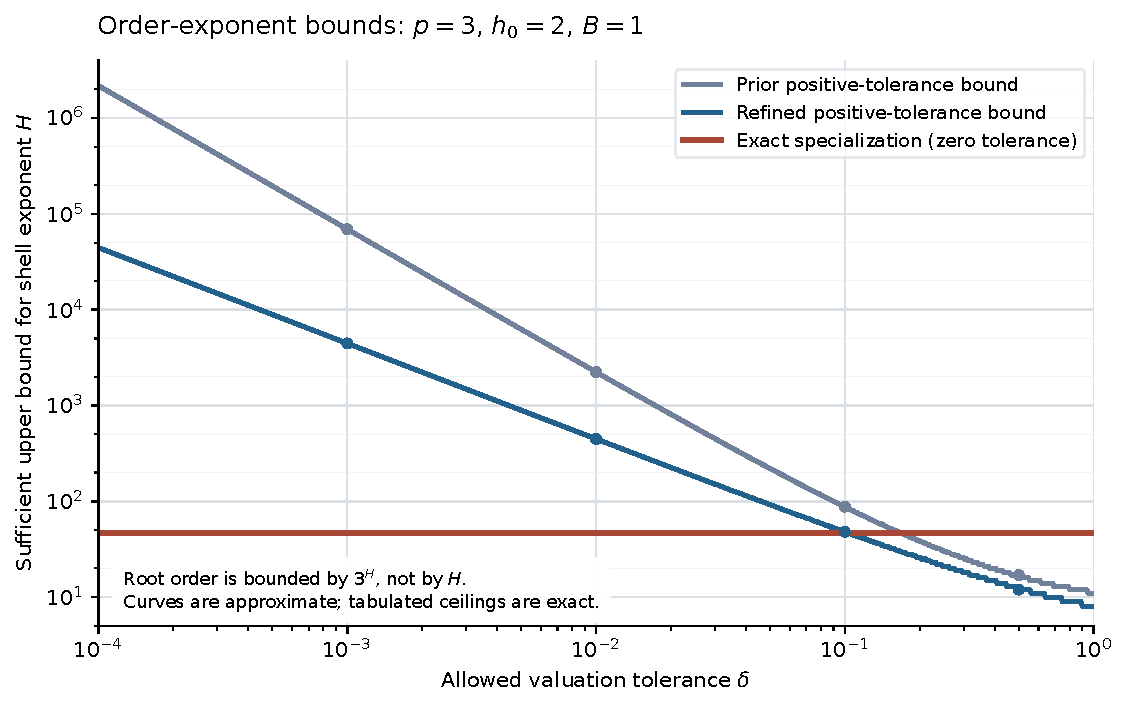
\includegraphics[width=0.92\linewidth]{figures/order_bounds.pdf}
\caption{Comparison of sufficient shell-exponent bounds for one function.
The plotted curves visualize the displayed formulas; the accompanying
table is computed with exact rational and integer-root arithmetic.
No empirical \(p\)-adic or prime-distribution data are used.}
\label{fig:bounds}
\end{figure}

\subsection{Twists and nonvanishing: a precise conditional use}

Suppose a particular arithmetic problem provides bounded integral
interpolation functions \(F_i(\mathbf T)\) whose values at torsion
parameters equal normalized special values or determinants, up to
explicit nonzero factors. Suppose it also provides nonzero witness values
with a total valuation budget \(B\). The theorem then selects a common
finite-order parameter at which all those interpolated values are nonzero
and their total valuation is at most \(B\). The first-powers construction
in Section~\ref{sec:exact-torsion} handles a finite list of powers of the
same parameter. If every first \(m\) power must be nontrivial, choose
\(p^{h_0}>m\).

This statement is useful only once the interpolation formula, integrality,
and witnesses are established. It is not a proof of nonvanishing when
the functions themselves are identically zero, when their coefficients
are unbounded, or when the chosen parameter space is not the allowed
arithmetic family. A bound on character order also does not bound the
norm of its conductor: the latter depends on where the character
ramifies and on the global realization of the local parameters.

There is substantial prior work on this subject. Kriz--Nordentoft
prove exact finite-group maximum-modulus principles and simultaneous
nonvanishing applications for horizontal \(p\)-adic \(L\)-functions
\cite{kn}. The exact comparison itself is therefore not a new general
phenomenon. Serban studies near-zero formal torsion loci, with
function-dependent thresholds under appropriate coefficient hypotheses
\cite{serban}. Schefer uses nearest-root arguments and cyclotomic distance
sums in quantitative torsion equidistribution; its bounds involve degree
and a polynomial-dependent separation constant \cite{schefer}.

The distinctive statement established here is the explicit order interval
depending only on a \emph{positive-radius Gauss budget}, uniformly in degree,
coefficient field, and number of coordinates. We did not locate this
particular bound in those primary sources. This targeted comparison is
not a proof of historical priority, and the theorem should not be
advertised as settling a previously named nonvanishing conjecture.

\subsection{Further restrictions that cannot be dropped}

The comparison radius must be positive. For \(F(T)=T\),
\(\G_0(F)=0\), while every nontrivial \(p\)-power root of unity has
\(v(F(\zeta-1))>0\). Thus an exact comparison with the coefficient
infimum at radius zero is false.

The coefficients must be bounded below in valuation. The series
\(\log(1+T)=\sum_{n\ge1}(-1)^{n+1}T^n/n\) converges on the open
unit disc and vanishes at every \(p\)-power torsion point shifted by
\(-1\), but its coefficients have unbounded negative valuations.
It is outside the theorem's hypotheses.

Finally, the theorem selects an order in an interval, not a prescribed
single shell. The integral polynomial \(\Phi_{p^H}(1+T)\) vanishes on
the entire primitive \(p^H\)-shell while its positive-radius Gauss
valuation is at most one. No universal assertion that the uppermost
shell itself works can hold under these hypotheses.


\section{Which open problems are realistic transfer targets?}
\label{sec:targets}

\subsection{Algebraic \texorpdfstring{\(K\)}{K}-groups: use the original strict estimate}

The original announcement explicitly points to a possible arithmetic
\(K\)-theory application of its Step 17 \cite{announcement}. This direction
is substantive because an internal Selmer bound contains information not
expressed by the final zero-location statement.

Two primary preprints already pursue it. Pintar's version-3 record states
vanishing of \(K_{4k}(\Z)\) through degree \(104\), conditional on the
original Step-17 arithmetic construction and its stated comparison route
\cite{pintar}. Mok--Zheng's 24 November preprint claims unconditional
vanishing through degree \(120\), while its provenance states that the
modified Gaussian Lean entry point has not been fully rebuilt
\cite{mokzheng}. These are distinct claims with distinct verification
conditions. We did not replay their complete arithmetic certificates,
reconstruct their large matrices, or compile the relevant original
dependency closure.

The shortened repository uses another route. Its theorem
\src{exists\_length\_shaOdd\_le} fixes a CM field \(E\subseteq\Q(\mu_N)\)
and a twist cutoff \(t\), then supplies a nonzero integer \(X\) bounding
certain odd-cocycle lengths by \(v(X)\), uniformly over finite coefficient
levels. Its introductory documentation does not identify that cocycle
model with the usual cohomological \(\Sha^1\). Its bound includes \(h_E\),
and the integer \(X\) is chosen after fixing \(E,N,t\)
\cite{oddsha}.

More decisively, the denominator proof and auxiliary-prime construction
explicitly avoid needing bounds for the even class groups where
Vandiver's conjecture lies \cite{denominator,triangle}. Avoiding their
contribution to a denominator estimate is different from proving that
they vanish. This distinction was already made in the preceding ProveIt
reports; we confirm it from the pinned source.

An elementary parity calculation explains the obstruction. Let
\(z:G\to M\) be a one-cocycle, and let \(c^2=1\) act trivially on \(M\),
where multiplication by two is injective. Then
\[
 0=z(c^2)=2z(c),\qquad
 z(chc)=z(c)+c\,z(h)+ch\,z(c)=z(h).
\]
So a rational cocycle for an even inverse cyclotomic twist at an odd
coefficient prime restricts to the even conjugation sector. The
shortened model's nonzero-twist condition selects the opposite sign.
Their intersection is zero. A duality or reflection argument might relate
other groups or twists, but such an argument is additional mathematics.

Other inferences also require care. A length bound by \(v(X)>0\) is not
vanishing; a length bound is not cyclicity; and replacing the fixed field
by \(E=\Q(\mu_\ell)\) as \(\ell\) varies destroys the original uniform
quantifier order. The general all-degree \(K_{4k}(\Z)\) vanishing question
is tied to Vandiver, as explained in Weibel \cite{weibel}. Cyclicity in
small degrees congruent to \(2\pmod4\) should not be billed as new:
the same reference already records a much larger classical range.

\subsubsection*{The original interface and the finite certificate}

The original archive has a stronger relevant term,
\path{UpperTheory.V.Z.J.OneCharU_s}.
It is used through \path{SmallClassNumbers/CorGKOf.lean}.
Schematically, subject to its full admissibility and nonzero-difference
hypotheses,
\[
 \forall \sigma\quad\exists X_\sigma\text{ finite}:\qquad
 V_n\le2\sum_{\pi\in X_\sigma}
       v_\ell\bigl(\operatorname{tr}\pi(\sigma)-t_\sigma\bigr).
\]
The witnesses can depend on the Frobenius probe \(\sigma\)
\cite{original}. Nothing in this quantifier order supplies one
representation working simultaneously at all probes.

Suppose exact integral branch determinants \(D_{q,j}\) have been justified
so that a surviving obstruction forces some \(D_{q,j}\) to be divisible
by \(\ell\), for every permitted probe \(q\). Then
\[
 \text{obstruction}\ne0
 \quad\Longrightarrow\quad
 \ell\mid\gcd_q\prod_jD_{q,j}.
\]
Indeed, at each \(q\) one factor is divisible, so its product is;
divisibility at every \(q\) passes to the gcd. Products must be taken
before the gcd because the witness branch may change.

The substantial input is the spectral coverage theorem: every admissible
trace difference, with its local type and normalization, must occur in a
shifted integral Hecke matrix or a valid coefficient norm. An exact gcd
alone does not establish this coverage. The nonzero-difference premise
must also remain attached to the original estimate.

The earlier ProveIt package already prepares Bernoulli-unit screening
and dimensions for degrees \(124\) and \(128\)
\cite{priormean}. A meaningful next step would be a fully justified
new large Hecke calculation for, for example, \(K_{124}(\Z)\),
after replaying the original Selmer bridge. This is beyond the range
of the located preprint, not a claim that the search certifies the first
currently unknown degree. The present report supplies no such matrix
and asserts no vanishing in these degrees.

\subsection{A nonabelian RH benchmark with an explicit remaining inequality}

Let \(L\) be the splitting field of \(X^3-X-1\), a degree-six
\(S_3\)-extension with quadratic subfield \(\Q(\sqrt{-23})\).
The earlier reports use this as a first nonabelian target
\cite{priormean,priorfoundations}. It is also the Hilbert class field
of that quadratic field. Its zeta function has a genuinely degree-two
class-character factor over \(\Q\), in addition to Dirichlet factors.
Dirichlet GRH does not directly settle that factor.

Write
\[
 -\frac{\zeta_L'}{\zeta_L}(s)=\sum_{n\ge2}\Lambda_L(n)n^{-s},
 \qquad
 \zeta_L(s)=\frac{\kappa_L}{s-1}
                +\kappa_L\gamma_L+O(s-1),
\]
and define
\[
 R_L(x)=\sum_{n\le x}\Lambda_L(n)\left(\frac1n-\frac1x\right)
              -\log x+\gamma_L+1.
\]
Here \(0\le\Lambda_L(n)\le6\Lambda(n)\).
For \(\Rea s>1\), termwise integration gives
\[
 \int_1^\infty R_L(x)x^{-s}\,dx
 =\frac{-\zeta_L'(s)/\zeta_L(s)}{s(s-1)}
    -\frac1{(s-1)^2}+\frac{\gamma_L+1}{s-1}.
\]
The subtractions remove the singularity at one. A nontrivial zero
\(\rho\) of multiplicity \(m_\rho\) gives residue
\(m_\rho/[\rho(1-\rho)]\), positive at real zeros in the critical strip.

The earlier positive-part Landau criterion therefore shows that
\[
 \boxed{\qquad
 \int_X^{2X}(R_L(x))_+\,dx
        \ll_\varepsilon X^{1/2+\varepsilon}
 \quad\text{for every }\varepsilon>0
 \qquad}                                           \tag{NB}
\]
would prove RH for \(\zeta_L\). The analytic proof uses the holomorphic
Mellin transform of the positive part, subtracts it from the meromorphic
transform, and applies the singularity theorem for a nonnegative
transform at its abscissa of convergence. Functional symmetry then gives
the full critical-line conclusion. The same fixed-field RH supplies
standard smoothed estimates in the other direction. Thus (NB) is a
reformulation with a potentially convenient arithmetic shape, not a
weaker conjecture already proved by the source.

To obtain (NB) by the source's method, one needs a lattice whose local
divisibility detects the new ideal-class or Frobenius statistic, enough
independent short forms, a determinant lower bound for that same
lattice, and total normalized errors of the required mean size.
The torsion theorem can help an aggregate denominator step if these
objects are available. It does not manufacture their divisibility or
their spanning.

This explains why changing the type of character in the Lean
source is not automatically an extension to nonabelian RH. The present
CM/cyclotomic construction encodes a specific arithmetic coefficient.
A new nonabelian coefficient must enter at that arithmetic stage.
The same issue persists in automorphic RH, with further local integrality
and representation-theoretic obligations.

\subsection{A focused research sequence}

A productive continuation has three milestones.

\begin{enumerate}[leftmargin=*,itemsep=5pt]
\item \textbf{Formalize the exact local theorem.}
Reuse the upstream root-radius, root-count, and Gauss-valuation lemmas;
formalize the two-state recurrence; then port the coefficient-selection
and tail arguments. Export the exact aggregate proposition with its
constant and its counterexamples. This is a finite, well-specified
formalization project whose mathematical gap has been closed here.
\item \textbf{Test one genuine arithmetic caller.}
Find a denominator estimate whose hypothesis is a total sum of normalized
lengths. Supply integral interpolation matrices and witness bounds.
If the caller instead requires individual budgets, retain the source
selector and do not substitute the aggregate theorem. Prove the global
character-realization and first-power conditions separately.
\item \textbf{Choose one open endpoint.}
For the finite \(K\)-theory route, validate the original strict
Selmer interface and a new exact Hecke certificate. For the nonabelian
RH route, prove the local divisibility identity for the cubic benchmark
before attempting the full theta-lift chain. A successful local lemma
would demonstrate that the new Frobenius information is really present.
\end{enumerate}

The arithmetic \(K\)-theory route has evidence of concrete finite
applications in the recent literature. The local torsion refinement is
ready for formalization and arithmetic testing. Nonabelian RH remains
a deeper geometric transfer, with an explicit missing inequality rather
than an asserted resolution.


\section{Verification, reproducibility, and the Lean boundary}
\label{sec:verification}

The general mathematical assertions are proved in
Section~\ref{sec:exact-torsion}. Two independent exact-arithmetic checkers
support that proof. They do not numerically approximate \(p\)-adic
distances: if two roots belong to a compatible \(p\)-power cyclotomic
tower, the valuation of their difference is computed from the order of
their ratio, using rational numbers.

The main checker verifies \(309\) recurrence configurations, \(60\)
capped-shell averages, \(405\) factored-polynomial examples, and nine
packets exhibiting the two false strengthenings. A separately written
checker verifies \(1{,}440\) recurrence steps, \(800\) polynomial cases,
and \(255\) torsion points in the dyadic obstruction. The edge cases
include \(B=0\), \(p=2,h_0=1\), exact zeros, roots at zero, and integral
factors with roots of negative valuation. The attached JSON files record
the precise finite scopes.

The proof review independently checked the cap at \(B+1\), the positive
state-matrix comparison, the discrete first-shell seed, the Gauss
coefficient induction, and preservation of exact valuations under
series truncation. An independent review is a useful mathematical check;
it is not a claim of journal review or kernel verification.

\subsection{Reproduce the supplied checks}

From the top directory of the extracted archive, run:
\begin{verbatim}
python3 checks/verify_exact_torsion.py
python3 checks/referee_exact_shell.py
python3 checks/compare_bounds.py
latexmk -pdf -interaction=nonstopmode -halt-on-error report.tex
\end{verbatim}
The first two scripts require only the Python standard library.
The plotting script additionally uses NumPy and Matplotlib; its numerical
curves are for visualization, while the table uses exact rational arithmetic
and integer square-root ceilings. LaTeX uses standard packages listed in
the preamble. The PDF was compiled and visually inspected before delivery.

The archive supplies an exact prior-archive inventory and source hashes,
proof-review notes, a bounded literature comparison, the complete \LaTeX\
source, the compiled PDF, checker code, outputs, plot data, and build
instructions. It does not duplicate all 26 incoming archives or the
entire upstream proof. The source manifests identify the inspected versions.

\subsection{A formalization plan with explicit obligations}

The numerical recurrence is the cleanest first Lean target. With
\(q=1/p\), \(c=1-q\), \(t>0\), set
\[
 u=Q/t,\quad z'=qz+u,\quad Q'=Q+cz',\quad
 u'=Q'/(t+1),\quad d=u-cz.
\]
Over a field, the two identities
\[
 u'-u=-\frac{qd}{t+1},\qquad
 u'-cz'=\frac{qt}{t+1}d
\]
are rational algebra. Positivity then proves componentwise comparison
and monotonicity for the negative-defect seed. These facts can be proved
without importing any RH statement.

The next layer should reuse the upstream definitions
\src{rootRadius}, \src{rootsOfValuation}, \src{gaussVal}, and
\src{ellVal\_eval\_add\_card\_mul}. New lemmas retain the exact
old-shell contribution \(W_{h-1}-p^{-1}z_{h-1}\), rather than only its
coarse fractional bound. The discrete seed is a positive multiset
cardinality. One should state carefully which valuation is truncated:
the mathematics here uses the ordinary additive valuation, while
the source's \src{ellVal} is clipped at zero; all selected points and
evaluated integral polynomials lie in the valuation ring, where the
values agree.

Only after the scalar theorem is checked should the multivariate
minimum-coefficient induction, bounded-series truncation, aggregate
product, and normalized matrix-length corollaries be added. Formalizing
the arithmetic realization of twists is a separate task. No Lean file
with placeholders is presented as a completed proof in this archive.


\appendix
\section{Comparison with the incoming corpus}
\label{sec:corpus}

The attached inventory identifies all 26 ZIPs at the pinned revision,
including duplicate-looking names with different suffixes. The following
grouping records what was used to avoid rediscovering already-developed
directions. Exact filenames, SHA-256 values, Git blob hashes, and manuscript
paths are in \path{evidence/prior_inventory.json}.

\begin{longtable}{@{}p{0.33\linewidth}p{0.61\linewidth}@{}}
\toprule
Report family & Material already present\\
\midrule
\endhead
Foundational transfer analyses & Source architecture, one-sided Mellin
criteria, cubic benchmarks, and original-versus-short source caveats.\\
Three method-transfer versions & Sparse sampling and ramification budgets;
bounded series and countable families; averaged criteria and exact
preparatory \(K\)-theory calculations.\\
Beyond-Dirichlet and quantitative-twists packages & Radial nonvanishing;
full power-series approximation; odd-cohomology comparison; polynomial
shell bounds with individual tolerances and good fractions.\\
Relative races and positive deficits & Relative zeta products, tower
compression, finite differences, averaged positive-part detectors, and
nonnegative Frobenius representatives modulo abelian functions.\\
Sylow, cyclic-generator, reflection, \(A_6\), and
\(\mathrm{PSL}_2\) packages & General finite-group detectors and sparse
conjugacy patterns, with degree/support calculations.\\
Kummer-window package & Prime-index Kummer criteria, an Artin--Hooley
density reduction, and shorter logarithmic auxiliary windows.\\
Arithmetic, exponent-six, CM, and singular-moduli packages &
Classifications, sparse relations, isogeny/prime applications, and
additional finite computations. These were inventoried; all their
certificates were not independently replayed.\\
Dirichlet-GRH research package & Heavenly abelian varieties, cubic
finiteness, critical-line Euler-product refinements, and progressions.\\
\bottomrule
\end{longtable}

No contradiction was identified in the targeted predecessor proofs
examined here. The main addition is the exact fixed-radius aggregate
specialization theorem and its explicit bound, together with the
counterexamples delimiting its scope. The one-sided nonabelian criterion
and the \(K\)-theory distinctions are retained as relevant prior
work rather than presented as new theorems.

\section{Related primary literature}
\label{sec:literature}

The comparison with \cite{kn,serban,schefer} is deliberately narrow.
Kriz--Nordentoft's Propositions 2.7 and 2.11 give exact finite-group
maximum-modulus principles; their Theorem 2.8 provides an
epsilon approximation after twisting by a finite exceptional set.
Serban's Proposition 2.8 and Lemma 2.9 concern near-zero torsion loci
and a discrete-coefficient threshold. Schefer's one-variable estimates
use the same broad nearest-root and ultrametric ideas but retain a
degree and separation-constant dependence.

These works are genuine antecedents. Our existence bound does not
recover their geometric classifications or equidistribution theorems.
The limited literature search found no identical
\(h_0+\lceil p^{h_0}B(h_0+B+2)\rceil\) budget-only statement;
absence from a limited search establishes no priority.


\begin{thebibliography}{99}
\raggedright
\bibitem{repo}
L. Sernau and collaborators,
\emph{GRH for Dirichlet \(L\)-functions, in Lean 4}, 2026.
\href{https://github.com/lsernau/grh-lean/tree/72fead102f663d5c7a407964a13dc0cf9d977207}{Pinned repository}.
The full commit and file hashes are recorded in this archive.

\bibitem{statements}
Same repository, \path{grh/src/Statements.lean} and
\path{grh/src/Main.lean}.
\href{https://github.com/lsernau/grh-lean/blob/72fead102f663d5c7a407964a13dc0cf9d977207/grh/src/Statements.lean}{Exact endpoint definitions}.

\bibitem{mainineq}
Same repository, \path{grh/src/New/Reduction/MainInequality.lean},
especially \path{star_inequality}.
\href{https://github.com/lsernau/grh-lean/blob/72fead102f663d5c7a407964a13dc0cf9d977207/grh/src/New/Reduction/MainInequality.lean}{Pinned source}.

\bibitem{onesided}
Same repository, \path{grh/src/New/Reduction/OneSidedBound.lean}.
\href{https://github.com/lsernau/grh-lean/blob/72fead102f663d5c7a407964a13dc0cf9d977207/grh/src/New/Reduction/OneSidedBound.lean}{Pinned source}.
See also \path{grh/GUIDE.md}.

\bibitem{criterion}
Same repository, \path{grh/src/New/Reduction/Zeros/Criterion.lean}.
\href{https://github.com/lsernau/grh-lean/blob/72fead102f663d5c7a407964a13dc0cf9d977207/grh/src/New/Reduction/Zeros/Criterion.lean}{Pinned source}.

\bibitem{landau}
Same repository, \path{grh/src/Lib/Analytic/Landau.lean}.
\href{https://github.com/lsernau/grh-lean/blob/72fead102f663d5c7a407964a13dc0cf9d977207/grh/src/Lib/Analytic/Landau.lean}{Pinned source}, in particular the nonnegative-transform and \path{IsPolar.landau} interfaces.

\bibitem{roots}
Same repository, \path{grh/src/New/Congruences/Selmer/RootsOfUnity.lean}.
\href{https://github.com/lsernau/grh-lean/blob/72fead102f663d5c7a407964a13dc0cf9d977207/grh/src/New/Congruences/Selmer/RootsOfUnity.lean}{Pinned source}.
Scalar selector at line 300; multivariate selector at line 474 in
the inspected revision.

\bibitem{oddsha}
Same repository, \path{grh/src/Lib/Cyclotomic/OddSha.lean}.
\href{https://github.com/lsernau/grh-lean/blob/72fead102f663d5c7a407964a13dc0cf9d977207/grh/src/Lib/Cyclotomic/OddSha.lean}{Pinned source}.

\bibitem{denominator}
Same repository, \path{grh/src/New/Congruences/FirstOrder/DenominatorBound.lean}.
\href{https://github.com/lsernau/grh-lean/blob/72fead102f663d5c7a407964a13dc0cf9d977207/grh/src/New/Congruences/FirstOrder/DenominatorBound.lean}{Pinned source}.

\bibitem{triangle}
Same repository, \path{grh/src/New/Congruences/FirstOrder/TrianglePrimes.lean}.
\href{https://github.com/lsernau/grh-lean/blob/72fead102f663d5c7a407964a13dc0cf9d977207/grh/src/New/Congruences/FirstOrder/TrianglePrimes.lean}{Pinned source}.

\bibitem{announcement}
L. Alp\"oge, \emph{A remark on the Riemann hypothesis}, November 2026.
\url{https://alpo.ge/remark.pdf}. Step 17 and footnote 6 concern the
original proof archive.

\bibitem{original}
Alp\"oge--Claude original development, mirror
\path{CocoSgt/riemann-hypothesis-lean}, revision
\texttt{7cbf7a0c32fca1badf05931879a37c3f8a2b03b4}.
\href{https://github.com/CocoSgt/riemann-hypothesis-lean/blob/7cbf7a0c32fca1badf05931879a37c3f8a2b03b4/src/Development/AutomorphicArithmetic/AutomorphicVarieties/SmallClassNumbers/CorGKOf.lean}{\path{CorGKOf.lean}} and
\href{https://github.com/CocoSgt/riemann-hypothesis-lean/blob/7cbf7a0c32fca1badf05931879a37c3f8a2b03b4/src/Development/AutomorphicArithmetic/AutomorphicVarieties/ModularityArgument/ThresholdArguments/DenseThresholdCases/NumberU3US.lean}{\path{NumberU3US.lean}}.

\bibitem{mokzheng}
C. P. Mok and H. Zheng,
\emph{Vanishing of \(K_{4m}(\mathbb Z)\) through degree \(120\)},
Hexagon 2611.00998v1, 24 November 2026.
\url{https://hexagonmath.org/2611.00998v1}.
Consult the provenance statement as well as the claimed theorem.

\bibitem{pintar}
L. Pintar, \emph{Vanishing of \(K_{4k}(\mathbb Z)\) through degree 104
from Alp\"oge's Step 17}, Hexagon 2611.00829v3.
\url{https://hexagonmath.org/2611.00829v3}.
The abstract retains the Step-17 arithmetic-construction assumption.

\bibitem{weibel}
C. A. Weibel, \emph{The \(K\)-book: An Introduction to Algebraic
\(K\)-theory}, Graduate Studies in Mathematics 145, AMS, 2013.
Chapter VI, Sections 9--10.
\url{https://sites.math.rutgers.edu/~weibel/Kbook/Kbook.VI.pdf}.

\bibitem{kn}
D. Kriz and A. C. Nordentoft, \emph{Horizontal \(p\)-adic \(L\)-functions},
arXiv:2310.20678v3. Propositions 2.7 and 2.11, Theorem 2.8.
\url{https://arxiv.org/html/2310.20678v3}.

\bibitem{serban}
V. Serban, \emph{An infinitesimal \(p\)-adic multiplicative
Manin--Mumford Conjecture}, Journal de Th\'eorie des Nombres de Bordeaux
30 (2018), no. 2, 393--408. DOI: 10.5802/jtnb.1030.
\url{https://www.numdam.org/item/JTNB_2018__30_2_393_0.pdf}.

\bibitem{schefer}
G. Schefer, \emph{\(p\)-adic equidistribution and an application to
\(S\)-units}, arXiv:2410.24088v1.
\url{https://arxiv.org/html/2410.24088v1}.
Nearest-root and Gauss-norm comparisons in the univariate and
multivariate sections.

\bibitem{priorquant}
ProveIt incoming manuscript,
\emph{Beyond Dirichlet GRH: Polynomial Order-Exponent Bounds for
Simultaneous \(p\)-adic Twisting}, 25 November 2026.
Archive \path{grh_quantitative_twists_2026-11-25.zip}.
Git blob \texttt{3468e65ff562dd2f77b9322d2ca484925b3e721d}.
\href{https://github.com/VladimirReshetnikov/ProveIt/tree/6fe2c1bd450aa7f19eab17fb9a6e76170b4fce00/docs/incoming}{Pinned incoming directory}.

\bibitem{priormean}
ProveIt incoming manuscript package,
\path{grh_method_transfers_2026-11-25 (2).zip}.
Sections \path{mean_transfer.tex}, \path{mean_additions.tex},
and \path{ktheory.tex}.
Git blob \texttt{99260f4c34ed4c80c1c4fbc95f76a7d9cfc3554f}.
Same pinned incoming directory as \cite{priorquant}.

\bibitem{priorfoundations}
ProveIt incoming manuscripts,
\path{grh_transfer_analysis_2026-11-25.zip} and
\path{grh_beyond_dirichlet_grh_2026-11-25.zip}.
Git blobs \texttt{2ec837a7b74075f98caa840b11ed467dd3e11509}
and \texttt{345edba99b36eaaee15693d61346d90b223ccfa9}.
Full inventory and targeted-review scope are supplied in this archive.
\end{thebibliography}


\end{document}

